\documentclass[a4paper,12pt]{article}

% Поддержка русского языка
\usepackage[T2A]{fontenc}	% Кодировка
\usepackage[utf8]{inputenc}	% Кодировка исходного текста
\usepackage[english,russian]{babel}	% Локализация и переносы
\usepackage{cmap}	% Поиск и копирование в PDF
\usepackage{listings}
\usepackage{geometry}	% Поля
    \geometry{left=35mm, right=10mm, top=20mm, bottom=20mm}
\usepackage{graphicx}
    \graphicspath{ {./images/} }
\usepackage{pgfplots}


\begin{document}

    \thispagestyle{empty}	% Отключаем колонтитулы
    
    \begin{center}
	Санкт-Петербургский политехнический университет Петра Великого\\
	Институт компьютерных наук и технологий\\
	\bfseries{Высшая школа программной инженерии}
\end{center}

\vspace{20ex} % Задаем размер вертикального промежутка в явном виде
    
    
    \begin{center}
	\begin{huge} {\bfseries{\scshape Лабораторная работа 4}} \end{huge}
\end{center}

\vspace{30ex}

\noindent Выполнил\\
студент гр.13534/21\hfill \begin{minipage}{0.6\textwidth} \hfill Н.А.Русанов\end{minipage}

\vspace{3ex}

\noindent Преподаватель\hfill \begin{minipage} {0.6\textwidth}\hfill А.В.Петров\end{minipage}

\vspace{3ex}

\hfill \begin{minipage}{0.6\textwidth} \hfill «\underline{\hspace{1cm}}»\underline{\hspace{3cm}} 201\underline{\hspace{0.5cm}} г.\end{minipage}

\vfill

\begin{center}
	Санкт-Петербург\\ 
	2019
\end{center}
    \section*{Задание}


    На основе примера, демонстрирующего различные уровни оптимизации, написать
    сценарий, выполняющий следующие действия в цикле:

    Компиляцию вашего приложения, не интерактивно обрабатывающего
    данные на языке C/C++/Fortran/Objective C/Objective C++/Ada с ключами
    оптимизации:
    \begin{itemize}
        \item -O0
        \item -O1
        \item -O2
        \item -O3
        \item -Os
        \item Вычисление времени выполнения программы (time). Приложение без
    оптимизации должно работать по меньшей мере 20 с.
        \item Вычисление занимаемого исполняемым файлом дискового пространства (в
    байтах) (du).
    \end{itemize}

    \section*{Ход работы}
    В ходе лабораторной работы был написан сценарий script.sh(Листинг 1), выполняющий компиляцию и предлагающий пользователю выбрать ключи оптимизации программы, отображающий время выполнения и занимаемое диковое пространство.
    \begin{center}
        \lstinputlisting[language=bash, basicstyle=\tiny, numbers=left,stepnumber=1]{src/script.sh}
    \end{center}

    Был сформирован график, отображающий результат оптимизации программы. Результат представлен на рисунке 1 и рисунке 2
\clearpage

        \begin{figure}[!h]
            \centering
            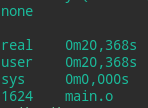
\includegraphics{none.png}
            \caption{ без оптимизации}
            
        \end{figure}   

        
        \begin{figure}[!h]
            \centering
            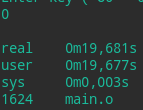
\includegraphics{O0.png}
            \caption{ оптимизация O0}
            
        \end{figure}   
        
        \begin{figure}[!h]  
            \centering
            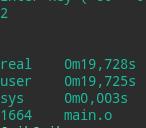
\includegraphics{O2.png}
            \caption{ оптимизация O2}
            
        \end{figure}   
        
        
        \begin{figure}[!h]
            \centering
            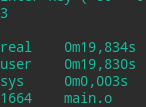
\includegraphics{O3.png}
            \caption{ оптимизация O3}
            
        \end{figure}   

        \begin{figure}[!h]
            \centering
            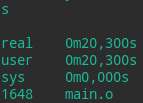
\includegraphics{OS.png}
            \caption{ оптимизация Os}
        \end{figure}   
          
 
       
        \begin{figure}[!th]  
              \centering
            \begin{tikzpicture}    
                \begin{axis}[
                        ymin=18,
                        ymax=21,
                        symbolic x coords={O0,O2,O3,none,OS},
                        xtick=data
                    ]
                        \addplot[ybar,fill=cyan] coordinates {
                            (O0,  19.681)
                            (O2,   19.728)
                            (O3,   19.834)
                            (none,   20.368)
                            (OS,   20.300)
                        };
                \end{axis}
                
            \end{tikzpicture}
            \caption{ график времени исполнения}
        \end{figure}
      
      
      
      \begin{figure}[!th]
            \centering
            \begin{tikzpicture}    
                    \begin{axis}[
                            ymin=1620,
                            ymax=1665,
                            symbolic x coords={O0,O2,O3,none,OS},
                            xtick=data
                        ]
                            \addplot[ybar,fill=cyan] coordinates {
                                (O0,  1624)
                                (O2,   1664)
                                (O3,   1664)
                                (none, 1624)
                                (OS,   1648)
                            };
                    \end{axis}
                    
                \end{tikzpicture}
            \caption{ Занимаемое дисковое пространство}
      \end{figure}
 
       \clearpage 
     
     \section*{Вывод}
     В ходе лабораторной работы был написан скрипт, позволяющий выбирать ключи оптимизации программы и выполняющий ее компиляцию.
    Было выявлено, что ключи оптимизации практически не влияют на выполнение программы, но изменяют размер исходного файла
    \end{document}

